\section{Preliminaries}\label{Section:Preliminaries}
%Need for handling uncertainty in data streams.
%BNs as the natural solution.

The following sections aim at describing some of the required concepts and basic structures to easily interpret the AMIDST models that will be presented afterwards for the different use cases. Section \ref{SubSection:HybridBNs} briefly introduces Bayesian networks and discuss the challenges encountered for reasoning with continuous and discrete variables, Section \ref{SubSection:DBNs} describes some of the basic concepts and models related to dynamic Bayesian reasoning over time, and finally, Section \ref{SubSection:DataAnalysis} defines the data analysis techniques used to support several assumptions made on the proposed models.

\subsection{Bayesian networks}\label{SubSection:HybridBNs}

Bayesian networks (BNs) \cite{JensenNielsen2007} are widely used probabilistic graphical models for reasoning under uncertainty. They graphically encode a set of conditional independence assumptions that are exploited to efficiently perform a wide variety of inference tasks such as marginal belief computation, belief updating, most probable explanation, etc.  

Formally, let $\bm X = \{X_1,\ldots,X_N\}$ denotes the set of stochastic random variables defining our domain problem. A BN defines a joint distribution $P(\bm X)$ in the following form:

$$ p(\bm X) = \prod_{i=1}^N p(X_i|Pa(X_i))$$ 

\noindent where $Pa(X_i)\subset \bm X\setminus X_i$ represents the so-called \emph{parent variables} of $X_i$. Bayesian networks can be graphically represented by a directed acyclic graph (DAG). Each node, labelled $X_i$ in the graph, encodes the factor or conditional probability $p(X_i|Pa(X_i))$ . Additionally, for each parent $X_j \in Pa(X_i)$, the graph contains one directed edge pointing from $X_j$ to the \emph{child} variable $X_i$.

Figure \ref{Figure:GeneralBayesianNetwork} contains an example of a BN model. The nodes are coloured to highlight the nature, discrete or continuous, of each variable according to the notation depicted in Figure \ref{Figure:PreliminariesNotation}. This is a very relevant aspect because it defines how each conditional probability $p(X_i|Pa(X_i))$ of the BN is defined. 

\begin{figure}
\begin{center}
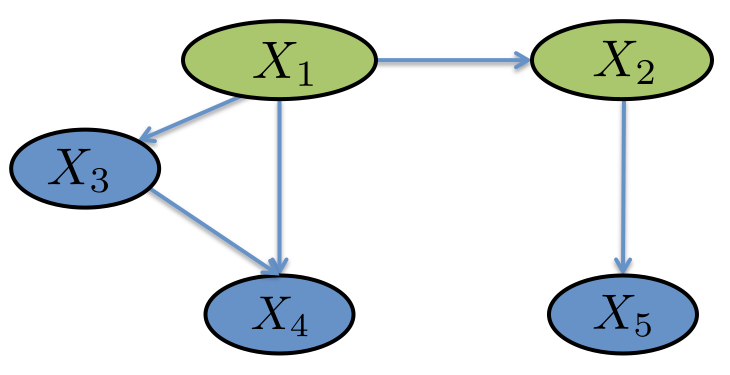
\includegraphics[scale=0.25]{./figures/GeneralBayesianNetwork}
\caption{\label{Figure:GeneralBayesianNetwork}Example of a Bayesian network with continuous and discrete variables.
}
\end{center}
\end{figure}


Traditionally, BNs have been defined for discrete domains, where the entities of interest are modelled by discrete variables which ensures that belief updating can be performed efficiently and in closed form. However, this requirement imposes severe restrictions as many domains contain entities that are more appropriately modelled by variables with continuous state spaces; such as distance and velocity measurements which are key sensor readings for identifying and interpreting traffic manoeuvres (see Daimler's requirement analysis \cite{Fer14}). 

To deal with this problem, research has been largely pursued on three main approaches to extend BNs and support continuous variables. As a first approach, one may choose to carefully construct the model so that exact inference algorithms can still be applied. This is the case for the conditional linear Gaussian (CLG) BNs \cite{Lauritzen1992,LauritzenJensen2001}, where the local probability distributions of continuous variables are specified as conditional linear Gaussian distributions and discrete variables can only have discrete parents. However, CLG BNs still impose certain limitations on the domain being modelled, i.e., discrete variables cannot depend directly on a continuous variable, and each continuous variable must follow a conditional linear Gaussian distribution. A second approach consists of considering approximate algorithms for performing inference, allowing thereby arbitrary distributions to be associated with the BN model. Examples of this approach include the Gibbs sampler \cite{Geman1984, hrycej1990gibbs} and variational inference \cite{Jordan1999}. Finally, the third approach consists of ``transforming" the original BN model into an approximate model, for which exact inference algorithms can be applied. This can be achieved either by discretizing the continuous variables \cite{KozlovKollerUAI97} or using transformations with more expressive power, such as using mixtures of truncated exponentials \cite{Moral2001} or mixtures of truncated basis functions \cite{Langseth12}.

\begin{figure}
\begin{center}
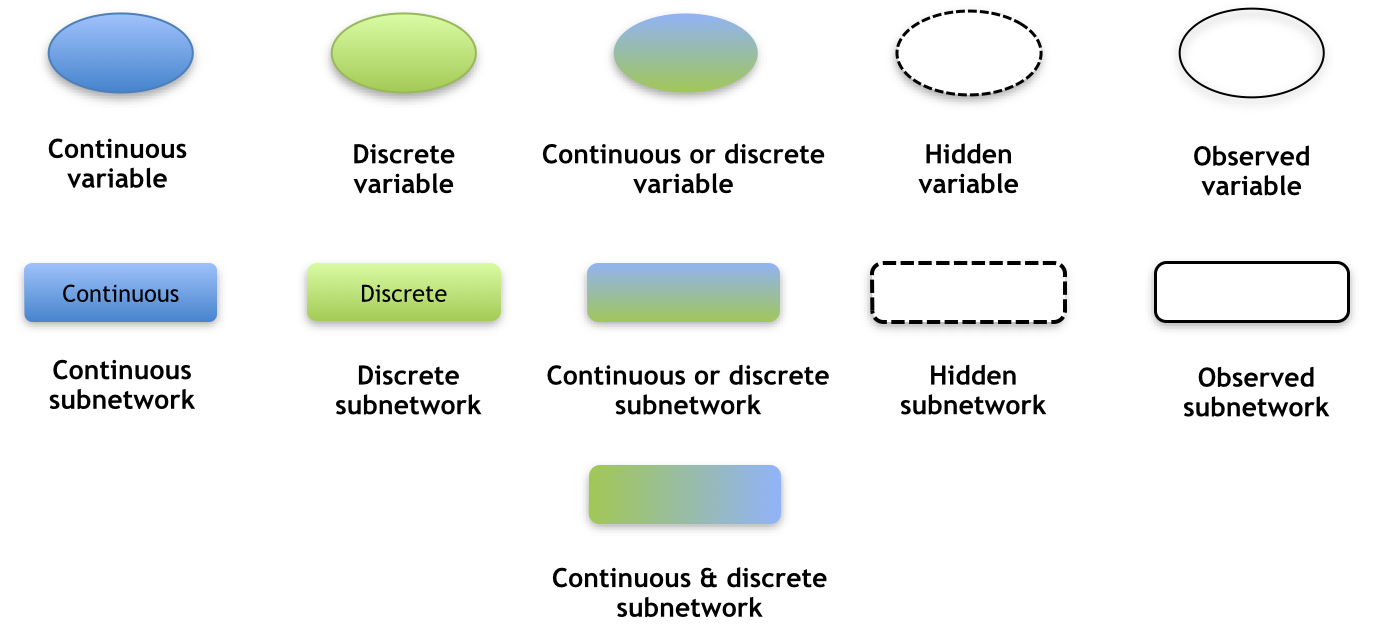
\includegraphics[scale=0.4]{./figures/PreliminariesNotation}
\caption{\label{Figure:PreliminariesNotation}Graphical notation of observed/hidden and continuous/discrete variables.
}
\end{center}
\end{figure}


\subsection{Probabilistic reasoning over time}\label{SubSection:DBNs}

Many domains, and in particular those being analysed in the AMIDST project, can be seen as having strong internal structure. This will be evident by the domains being appropriately described using an object oriented language, either due to repetitive substructures or substructures that can be naturally ordered in a superclass/subclass hierarchy.  Object oriented BNs \cite{KollerPfeffer1997} (OOBNs) are defined to take advantage of such internal model structure. In dynamic models, we also find this property because the same part of the model is repeated over time (i.e., we have multiple objects of the same class under the OOBNs language). A special type of OOBNs is the dynamic BN (DBN) \cite{DeanKanazawa1989}, which is used to model domains that evolve over time by representing explicitly the temporal dynamics of the system. DBNs can be also readily understood as an extension of standard BNs to the temporal domain. 

Similarly to static BNs, we model our problem/system using a set of stochastic random variables, denoted $\bm X_t$, with the main difference that variables are indexed here by a discrete time index $t$. In this way, we explicitly model the state of the system at any given time. Moreover, we always assume that the system is modelled at a fixed frequency, and use $\bm X_{a:b} \equiv X_a,X_{a+1},\ldots,X_{b}$ to denote the set of variables between two time points $a$ and $b$.  

For reasoning over time, we need to model the joint probability $p(\bm X_{1:T})$ which has the following natural cascade decomposition:

$$p(\bm X_{1:T})  = \prod_{t=1}^T p(\bm X_t|\bm X_{1:t-1})$$

\noindent where $p(\bm X_t|\bm X_{1:t-1})$ is equal to $p(\bm X_1)$ for $t=1$. As $t$ increases, the conditional probability $p(\bm X_t|\bm X_{1:t-1})$ becomes intractable. Similarly to static BNs, \textit{dynamic BNs} allow more compact factorization of the above joint probability. The first conditional independence assumption encoded by DBNs to reduce the factorization complexity is the well-known \textit{Markov assumption}. Under this assumption, the current state is independent from the previous one given a finite number of previous steps. Dynamic models satisfying the Markov assumption are called \textit{Markov chains}. Basically, a Markov chain can be defined on either discrete or continuous variables $\bm X_{1:T}$. It exploits the following equality:

$$p(\bm X_t| \bm X_{1:t-1})  = p(\bm X_t|\bm X_{t-V:t-1})$$

\noindent where $V\geq 1$ is the order of the Markov chain. Figure \ref{Figure:markovChain} shows two examples of DBNs corresponding to first-order (i.e., $V=1$) and third-order (i.e., $V=3$) Markov chains. 

\begin{figure}[ht!]
\begin{center}
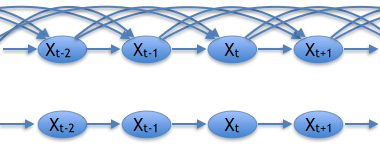
\includegraphics[scale=0.56]{./figures/PreliminariesMarkovChain}
\caption{\label{Figure:markovChain} An example of DBNs assuming a third-order Markov property (above) and a first-order Markov property (below).
}
\end{center}
\end{figure}

Among different kinds of Markov chains, the \textbf{first-order Markov chains} are the most widely used. They assume that knowing the present makes the future conditionally independent from the past, that is, $p(\bm X_t| \bm X_{1:t-1})  = p(\bm X_t|\bm X_{t-1})$. The problem is that this could be an unrealistic assumption in some problems leading to poor approximations of the joint distribution. Consequently, in order to increase the accuracy of the approximation, one could either increase the Markov order, or equivalently, increase the number of state variables, which would consequently increase the complexity. Hence, our objective is to come up with models that contain a self-sufficient set of variables, which likewise requires to fully understand the ``physics''  of the process being modelled for the different use cases \cite{russelNorvig2009}. 

An additional challenging problem is the specification of the conditional probabilities at each time step of the DBNs. To deal with this problem, we usually assume that changes in the world state are driven by a \textit{stationary process}, that is, $p(\bm X_{t+1}|\bm X_{t}) = p(\bm X_t|\bm X_{t-1})\ \forall t \in\{1,\ldots,T\}$. 

In the following sub-sections, we will present in more details some basic examples of DBNs, namely, \textit{hidden Markov models} (Section \ref{SubSubSection:HMMs}) and \textit{Kalman filters} (\ref{SubSubSection:KFs}). Moreover, in Section \ref{SubSubSection:2DBNs}, we will introduce the specific DBN model, mostly used in AMIDST, known as the \textit{two-time slice DBN}. Let us recall here that the graphical notation employed when describing all these models is depicted in Figure \ref{Figure:PreliminariesNotation}.
%Besides, distinctions are made between discrete and continuous ones, because they have a strong impact in the kind of model that we consider. 

%--------------------------
\subsubsection{Hidden Markov models}\label{SubSubSection:HMMs}
%--------------------------
A hidden Markov model (HMM) is the simplest DBN including both hidden and observed variables, such that the latent state of the process is represented by a single discrete variable. More precisely, a HMM defines a Markov chain on hidden (or non-observable) variables $X_{1:T}$. The observed variables, denoted by $\bm Y_{1:T}$, are dependent on the hidden variables under the \textit{sensor Markov assumption}, that is, $P(\bm Y_t| X_{1:T}, \bm Y_{1:t-1}) = P(\bm Y_t| X_t)$, where $P(\bm Y_t| X_t)$ represents the the sensor (or observation) model.  

\begin{figure}[ht!]
\begin{center}
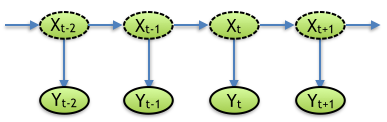
\includegraphics[scale=0.56]{./figures/PreliminariesHMM}
\caption{\label{Figure:HMM}An example of a BN structure corresponding to a HMM.}
\end{center}
\end{figure}

In that way, the joint probability distribution over the observed and hidden variables can be represented as:

\begin{equation}
P(\bm X_{1:T},\bm Y_{1:T}) = \prod_{t=1}^t{P(\bm X_t| \bm X_{t-1})P(\bm Y_t|\bm X_t)}
\end{equation}

Although most of our models will fit into this description of observed and hidden (state) variables, there will be cases in which the transition model takes place in the observed variables (the case of Cajamar), which in general simplifies the learning-inference processes of the problem.

%--------------------------
\subsubsection{Kalman filters}\label{SubSubSection:KFs}
%--------------------------
Similar to the extension of the static BN model to hybrid domains, DBNs have likewise been extended to continuous and hybrid domains. In purely continuous domains, where the continuous variables follow linear Gaussian distributions, the DBN corresponds to (a factorized version of) a Kalman filter (KF). The structure of a KF is exactly the same as the one displayed in Figure \ref{Figure:HMM} for the HMM, however with the restriction that all variables should be continuous. In this case, the state variables can be a combination of continuous variables with different dependences, and the dynamics of the process are assumed to be linear. 

When modelling non-linear domains, the dynamics and observational distributions are often approximated through, e.g., the \textit{extended Kalman filter}, which models the system as \textit{locally} linear in the mean of the current state distribution. In addition, in order to perform non-linear predictions, we need a more expressive model such as the \textit{switching Kalman filter} (SKF). The SKF includes an extra discrete state variable to the network that allows to model multiple KFs running in parallel. Figure \ref{Figure:SKF} depicts the graphical structure of this dynamic model.

\begin{figure}[ht!]
\begin{center}
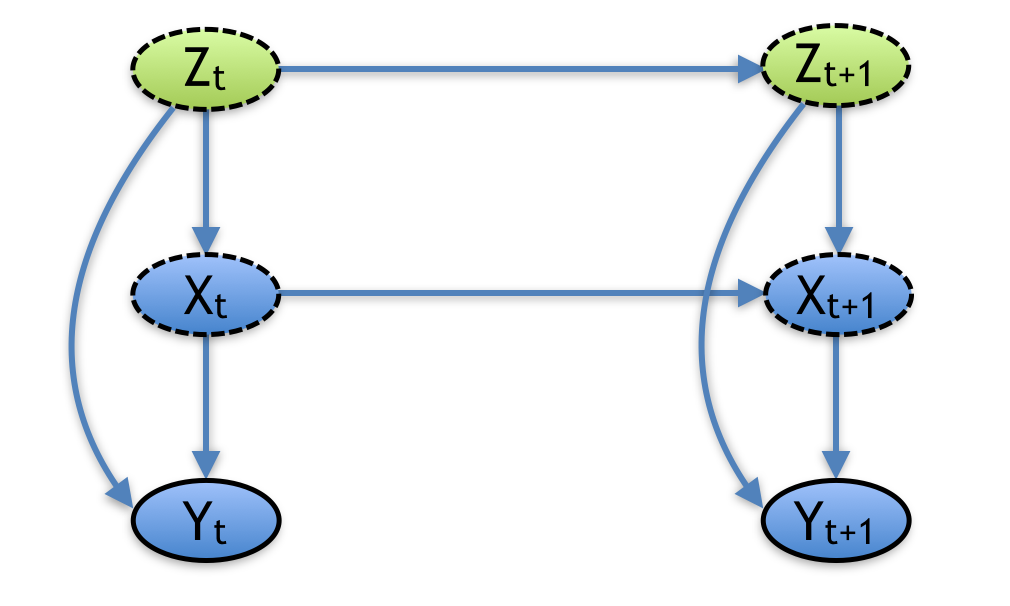
\includegraphics[scale=0.3]{./figures/SKF}
\caption{\label{Figure:SKF} A Switching Kalman Filter. $Z_t$ is the discrete state variable that allows to model multiple KFs running in parallel.}
\end{center}
\end{figure}

%--------------------------
\subsubsection{Two-time slice dynamic Bayesian networks}\label{SubSubSection:2DBNs}	
%--------------------------

In general, DBNs can model arbitrary distributions over time. However, in AMIDST,  we will especially focus on the so-called \textit{two-time slice DBNs} (2T-DBNs). 2T-DBNs are characterised by an \textit{initial model} representing the initial joint distribution of the process and a \textit{transition model} representing a standard BN repeated over time. This kind of DBN model satisfies both the first-order Markov assumption and the stationary property. Figure \ref{Figure:DBN} shows an example of a graphical structure of a 2T-DBN model. 

\begin{figure}[ht!]
\begin{center}
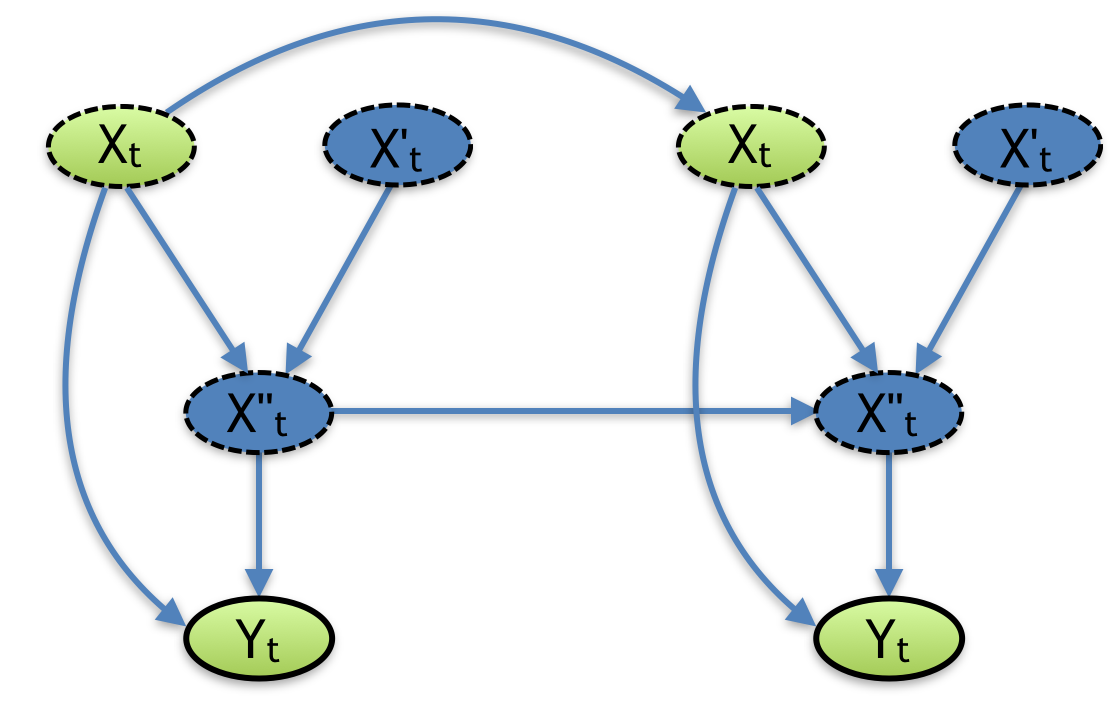
\includegraphics[scale=0.3]{./figures/PreliminariesDBN}
\caption{\label{Figure:DBN}An example of a BN structure corresponding to a 2T-DBN.}
\end{center}
\end{figure}

In a 2T-DBN, the transition distribution is represented as follows:

$$ p(\bm X_{t+1} | \bm X_t) = \prod_{X_{t+1}\in\bm X_{t+1}} p(X_{t+1}|Pa(X_{t+1}))$$ 

\noindent where $Pa(X_{t+1})$ refers to the set of parents of the variable $X_{t+1}$ in the transition model, which can be variables either at the same or the previous time step. 

Note that a HMM, KF or SKF are particular cases of a 2T-DBN. Equally, some 2T-DBNs could be casted to some of these standard models by grouping some variables. For example, the 2T-DBN shown in Figure \ref{Figure:DBN} can be considered as a SKF if we group $X_t$ and $X'_t$ by a cartesian product in a single and bigger variable $Z_t \equiv X_t \times X'_t $. However, It is usually preferred to factorise the transition distribution by taking the 2T-DBN graphical structure into account. This is due to the fact that we can take advantage of the sparseness of the model, especially when dealing with high-dimensional problems. For instance, in our considered example, the transition probability of the equivalent SKF model would be simply expressed as $p(Z_{t+1}|Z_t)$. However, by taking the 2T-DBN graphical structure into account, this transition probability could be much more compactly expressed as $p(Z_{t+1}|Z_t)=P(X'_{t+1})p(X_{t+1}|X_t)$.

DBNs obviously share the computational difficulties of regular BNs in inference tasks. However, in the dynamic case, we are also faced with the \textit{entanglement problem}, i.e., after a certain time step, all variables describing the current system state will become dependent, and we cannot therefore represent the exact probability distribution over the current state (the belief state) in a compact and factorized form. To deal with this problem, approximate methods (including approximate factorizations of the joint probability distribution describing the system state) \cite{BoyenKoller1998} as well as sampling based techniques in the form of particle filtering \cite{Doucet2000} are usually used.

%--------------------------
\subsection{Data analysis}\label{SubSection:DataAnalysis}
%--------------------------

%As already commented in the introduction
The motivation behind using data analysis is first to test some assumptions supporting the models elicited by the experts in the different use cases, and second, to further complement our understanding about the nature of the problem we are modelling. In the following sub-sections, we will introduce the set of tools, namely sample correlograms, sample partial correlograms, histograms, and bivariate distributions, that allows us to get insights into both structural and distributional DBN assumptions.

%--------------------------
\subsubsection{Sample correlograms and sample partial correlograms}
%--------------------------

A DBN mainly aims to model complex multivariate time series. By using sample correlograms and sample partial correlograms, we will try to test if the available data supports the temporal correlation between variables assumed by the DBN model, i.e., the temporal links between variables. However, these tools will only allow us to look at univariate time series, what strongly limits the extent of the extracted conclusions. However, despite its limitations, this analysis will give us some interesting insights which usually cannot be elicited from experts, as we will see below for the different use-cases.  

\begin{itemize}
\item \textbf{Sample correlograms}: Let ${x_1,...,x_T}$ be a univariate time series. The \emph{sample autocorrelation coefficient} at lag $v$ is given by 

$$ \hat{\rho}_v =\frac{\sum_{t=1}^{T-v} (x_t-\bar{x})(x_{t+v}-\bar{x})}{\sum_{t=1}^{n} (x_t-\bar{x})^2}$$ 

\noindent where $\bar{x}$ is the sample mean and $T$ is the total length of the considered data. The plot of $\hat{p}_v$ versus $v$, for $v=1,\ldots, M$ for some maximum $M$ is called the \emph{sample correlogram} of the data. $\hat{p}_v$ corresponds to the Pearson correlation between the series $\{x_t\}_{t\in\{1,...,T\}}$ and $\{x_{t+v}\}_{t+v\in\{1,...,T\}}$.

Sample correlograms can be interpreted as a way to measure the strength of the following unconditional dependences: $X_t  \not\perp X_{t+v}$ for some lag $v \geq 1$.  When $\hat{\rho}_v$ is close to zero, this indicates that there exists a strong unconditional independence between $X_t$ and $X_{t+v}$. However, when $\hat{\rho}_v$ is close to either $1$ or $-1$, this indicates that there is a strong correlation or dependency between $X_t$ and $X_{t+v}$. However, once again, we should never forget that when computing these Pearson correlation coefficients, we are making a strong assumption about the normality of the data, which might not hold in the data.

Figure \ref{Figure:PreliminariesCorrelograms} shows examples of sample correlograms for two different types of data sets: Figure \ref{Figure:PreliminariesCorrelograms}(a) shows a sample correlogram for a sequence of 50 i.i.d. data records sampled according to a Gaussian distribution with zero mean and unit variance $x_t\sim {\mathcal N}(0,1)$; and Figure \ref{Figure:PreliminariesCorrelograms}(b) shows a sample correlogram for a sequence of 50 data samples distributed as $x_t=x_{t-1} + \epsilon$, such that $\epsilon\sim {\mathcal N}(0,1)$. As it can be seen, the correlogram for the i.i.d. data has values close to zero for all lags. However, for time series data, the correlogram clearly identifies the presence of a temporal relationship in the data. As expected, the correlation decreases with the size of the lag, and how quickly it decreases depends on the strength of the temporal relationship. 


\item \textbf{Sample partial correlograms}: Let $X_t$ be a random variable associated to $X$ taking values at time $t$. We can build the following regression problem:

$$ X_t = a_0 + a_1X_{t-1} + a_2X_{t-2} + ... a_{v-1}X_{t-v-1}$$

In addition, let $e_{t,v}$ denotes the residuals of this regression problem (i.e., the error when estimating $X_t$ using a linear combination of $v-1$ previous observations). The \emph{sample partial auto-correlation coefficient} of lag $v$, denoted as  $\hat{\theta}_v$, is the standard sample auto-correlation between the series $\{x_{t-v}\}_{t-v\in\{1,...,T\}}$ and $\{e_{t,v}\}_{t\in\{1,...,T\}}$. Intuitively, the sample partial auto-correlation coefficient of lag $v$ can be seen as the correlation between $X_t$ and $X_{t+v}$ after having removed the common \emph{linear} effect of the data in between.

As previously, we plot in Figure \ref{Figure:PreliminariesCorrelograms} (c) and (d) the sample partial correlograms for the same two data sequences presented above. In the case of i.i.d. data, we can see again that the partial correlogram does not show any sign of partial correlation between the data sequence samples. However, for time series data, the partial correlogram takes a high value for $v=1$ (for this lag value it is equal to the sample correlogram), but then becomes close to zero for $v$ values higher than 1. The sample partial correlogram can be interpreted as a way to measure the strength of the following conditional dependence: $X_t  \not\perp X_{t+v} | X_1,...,X_{t+v-1}$ for some lag $v>1$. Accordingly, the sample partial correlogram correctly identifies that we have the following conditional independencies: $X_t\perp X_{t+2}|X_{t+1}$ in the considered time series data. 

Therefore, sample partial correlograms can be seen as a tool to test the order of the Markov chain generating the time data sequence, with all the same caveats expressed for the sample correlogram. 

\begin{figure}[ht!]
\begin{center}
\begin{tabular}{cc}
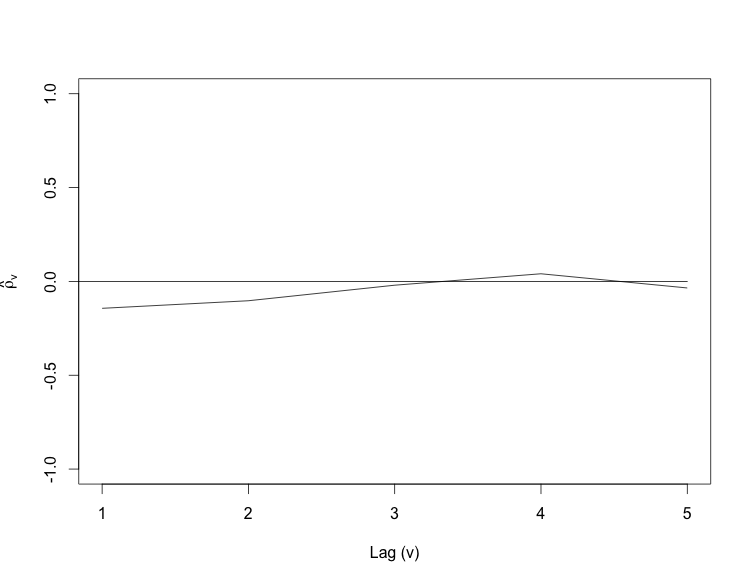
\includegraphics[scale=0.25]{./figures/CorrelogramGaussian} &
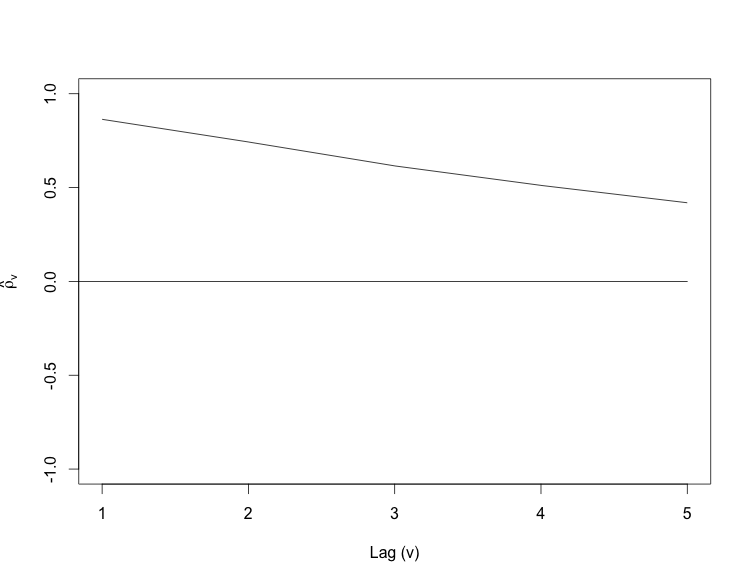
\includegraphics[scale=0.25]{./figures/CorrelogramTimeSerie} \\
\small (a) Correlogram for i.i.d. data & \small (b) Correlogram for a time series data \\
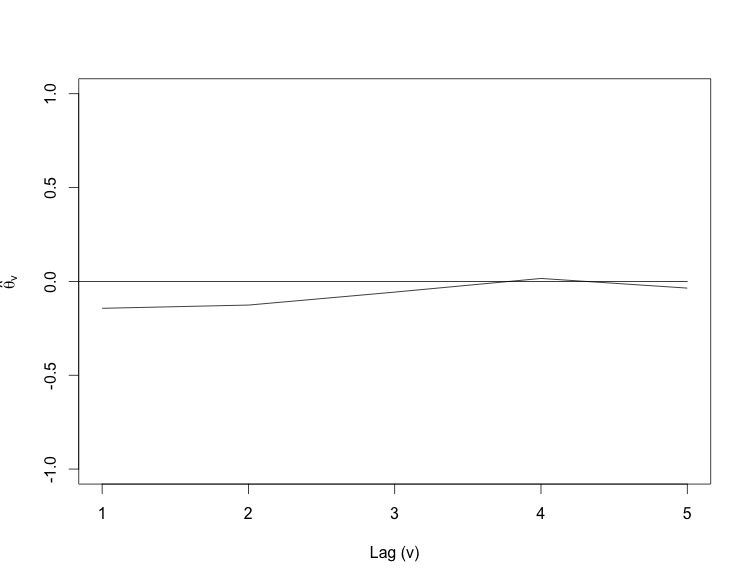
\includegraphics[scale=0.25]{./figures/PartialCorrelogramGaussian} &
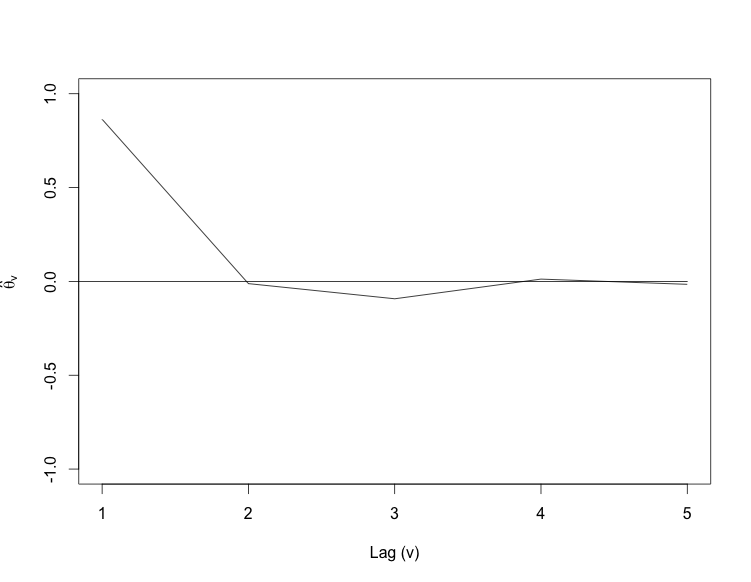
\includegraphics[scale=0.25]{./figures/PartialCorrelogramTimeSerie} \\
\small (c) Partial correlogram for i.i.d. data & (d) \small Partial correlogram for a time series data \\
\end{tabular}
\caption{\label{Figure:PreliminariesCorrelograms} Examples of sample correlograms and sample partial correlograms for i.i.d. and time series data. 
}
\end{center}
\end{figure}

\end{itemize}

\subsubsection{Histograms and bivariate contour plots}

The aim here is to use histograms and bivariate distributions in order to get insights into the conditional probability distributions of the proposed models. 

\begin{itemize}
\item \textbf{Histograms}: Despite the fact that this tool is quite useful in a static context, it is rather limited in dynamic models. For example, let assume we have a time series $x_1,\ldots, x_T$ and our histogram shows that the empirical distribution of the variable when we aggregate the data samples over time looks like a mixture of Gaussian distributions. In this case, there are two simple possibilities that can give rise to this finding: 
i) $X_t$ is distributed according to a mixture of Gaussians where each Gaussian component depends on $X_{t-1}$; and ii) there is a discrete hidden variable $Z_t$ that influences $X_{t}$ and is the one responsible for generating the different mixture components. 

However, despite its limitations in dynamic contexts, we will resort to the use of histograms whenever we find that they could shed some lights on the underlying sample distribution of the sample.
%As shown in this example, histograms are difficult to interpret in dynamic models, but we are going to use them when we think that they can be of some help. 

\item \textbf{Bivariate contour plots}: The contour plots of the empirical bivariate distribution of $X_t$ versus $X_{t-1}$ can show many relevant information, such as the presence of linear relationships between variables or if we can assume they are normally distributed, etc. In Figure \ref{Figure:PreliminariesBivariates}, we plot the bivariate contour plot for the i.i.d and time series data described above. As it can be seen, the bivariate contour plot for time series data shows how $X_t$ and $X_{t+1}$ seems to be distributed according to a bivariate normal with a covariance matrix that displays a strong degree of correlation. In the case of i.i.d. data, the bivariate contour plot does not reveal any temporal dependence between $X_t$ and $X_{t-1}$. 

\begin{figure} [ht!]
\begin{center}
\begin{tabular}{cc}
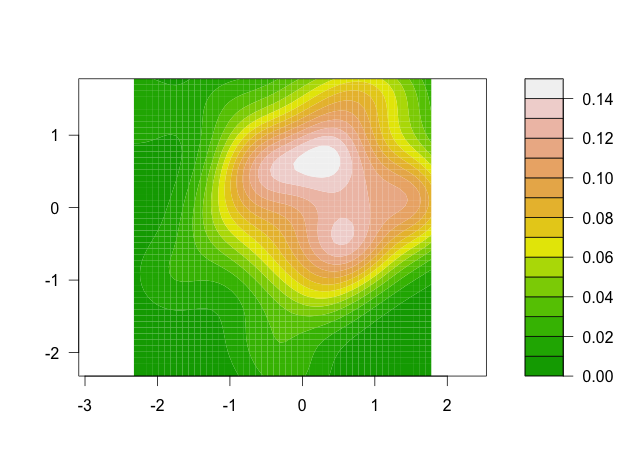
\includegraphics[scale=0.25]{./figures/BivariateGaussian} &
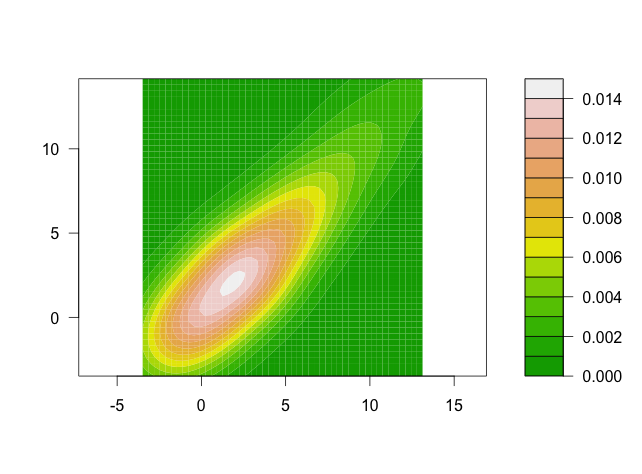
\includegraphics[scale=0.25]{./figures/BivariateTimeSerie} \\
(a) i.i.d. data & (b)  Time series data \\
\end{tabular}
\caption{\label{Figure:PreliminariesBivariates}Bivariate contour plots for a set of i.i.d. and time series data. 
}
\end{center}
\end{figure}

\end{itemize}

Finally, note that the usefulness of all these tools is limited due to its generative nature. That is, they do not explicitly target the prediction problem for the different use cases. After performing a proper evaluation of the considered static and dynamic models, it will be possible to re-adjust, if needed, our current assumptions. 
